\section{Constraints}

The constraints are implemented using a generic solver.
This method allows us to implement new constraints easily.
Each constraint is implement using the \verb"Constraint" interface.
This interface requires a constraint to have the following functions:
\begin{itemize}
  \item GetC\\
  \emph{ This function contains the constraint }
  \item GetCdot\\
  \emph{ This function contains the time derivative of the constraint }
  \item GetDerivative\\
  \emph{ This function contains the partial derivative of the constraint  }
  \item GetTimeDerivative\\
  \emph{ This function contains the partial time derivative of the constraint }
\end{itemize}

\begin{figure}[t]
  \centering
  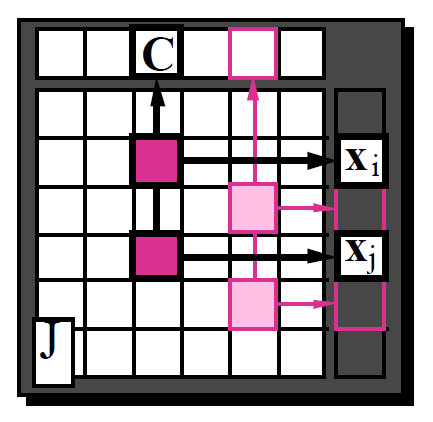
\includegraphics[width=5cm]{img/jacobian.png}
  \captionof{figure}{Visualisation of the jacobian matrix}
  \label{fig:jacobian}
\end{figure}

\noindent To resolve all constraints the following matrices are calculated.
With these matrices the constrain forces for each particle are calculated.\\
$J$, the jacobian matrix.\\
\emph{We loop through all constraints and add their GetDerivative() values to the appropriate places in the matrix.
The resulting matrix has the structure as shown in Figure ~\ref{fig:jacobian}, where $C$ is a constraint and $x$ is a particle.}\\
$W$, inverse of the mass matrix\\
$\dot{J}$, jacobian time derivative matrix\\
\emph{Same as $J$, but uses GetTimeDeivative() instead of GetDerivative().}\\
$\dot{q}$, vector of all velocities\\
$Q$, vector of all constraint forces\\
$C$, vector of all constrains\\
$\dot{C}$, partial derivative of constraints vector $C$\\
\\
With these matrices we solve the following equation with a linear solver:\\
$Ax = B$ where\\
$A = J W J^{T}$\\
$B = (-\dot{J} \dot{q}^{T} - J W Q^{T}) - (C k_s) - (\dot{C} k_d)$\\
We added the feedback term $- (C k_s) - (\dot{C} k_d)$ to prevent drifting in the constraint force calculation.
With the calculated $x$ matrix we can calculate the constraint forces matrix using the formula $\hat{Q} = x^{T} J$.
The forces of each particles are updated using this resulting constraint forces matrix.\\

\subsection{Rod}
Used to constrain two particles $p_1 = (x_1,y_1)$ and $p_2 = (x_2,y_2)$ to be a fixed distance $r$ apart.
\begin{itemize}
  \item GetC: $C = (x_1 - x_2)^2 + (y_1 - y_2)^2 - r^2$
  \item GetCdot:\\
    $\dot{C} = {v_1}^T \frac{\partial C}{\partial p_1} + {v_2}^T \frac{\partial C}{\partial p_2}$
  \item GetDerivative:\\
    $\frac{\partial C}{\partial p_1} = 2 (p_1 - p_2)$\\
    $\frac{\partial C}{\partial p_2} = -2 (p_1 - p_2)$
  \item GetTimeDerivative:\\
    $\frac{\partial^2 C}{\partial p_1 \partial t} = 2 (v_1 - v_2)$\\
    $\frac{\partial^2 C}{\partial p_2 \partial t} = -2 (v_1 - v_2)$
\end{itemize}

\subsection{CircularWire}
Used to constrain a particle $p = (x, y)$ to be a fixed distance $r$ from some point $p_c = (x_c, y_c)$.
\begin{itemize}
  \item GetC: $C = (x - x_c)^2 + (y - y_c)^2 - r^2$
  \item GetCdot:\\
    $\dot{C} = {v}^T \frac{\partial C}{\partial p}$
  \item GetDerivative:\\
    $\frac{\partial C}{\partial p} = 2 (p - p_c)$
  \item GetTimeDerivative:\\
    $\frac{\partial^2 C}{\partial p \partial t} = 2 (v - v_c)$
\end{itemize}

\subsection{Fixed}
Used to constrain a particle $p = (x, y)$ to be a fixed point $p_c = (x_c, y_c)$.
This constraint has the same implementation as CircularWire, but with $r = 0$.

\subsection{Line}
Used to constrain a particle $p_L = (x_L, y_L)$ to be on a fixed horizontal or vertical line.
This line is defined by a point $p_1 = (x_1, y_1)$ and boolean $isHorizontal$.
Below the constraint of a horizontal line is described, the vertical line follows naturally.
\begin{itemize}
  \item GetC: $C = y_L - y_1$
  \item GetCdot:\\
    $\dot{C} = y_L$
  \item GetDerivative:\\
    $\frac{\partial C}{\partial p_L} = $
    $\bigl(\begin{smallmatrix}
    0\\ 1
    \end{smallmatrix} \bigr)$
  \item GetTimeDerivative:\\
    $\frac{\partial^2 C}{\partial p_L \partial t} = $
    $\bigl(\begin{smallmatrix}
    0\\ 0
    \end{smallmatrix} \bigr)$
\end{itemize}



